We compute the ground state of the TFI model \eqref{eq:TFI_Hamiltonian} using disoTPS and TEBD with imaginary time $\tau = -i t$. As initial state we choose the product state $\ket{\Psi_i}=\ket{\uparrow}\otimes\cdots\otimes\ket{\uparrow}$ of all spins pointing up. One can expand the initial state in terms of energy eigenstates
\begin{equation}
	\ket{\Psi_i} = \sum_{n} \Psi_n \ket{n}.
\end{equation}
Applying the time evolution and normalizing then leads to the state
\begin{equation}
	\ket{\Psi(t)} = e^{-i\tau\hat{H}} \ket{\Psi_i} = \frac{1}{\mathcal{N}} \sum_{n} \Psi_n e^{-iE_n\tau} \ket{n} = \frac{1}{\mathcal{N}} \sum_{n} \Psi_n e^{-E_nt} \ket{n}
\end{equation}
with
\begin{equation}
	\mathcal{N} = \left\lVert\sum_{n} \Psi_n e^{-E_nt}\right\rVert
\end{equation}
If we now take the limit $t \rightarrow \infty$ and assume that the ground state $\ket{0}$ with the lowest energy $E_0$ is nondegenerate, all states except the ground state vanish because of the exponential terms $e^{-E_nt}$. We end up with the ground state
\begin{equation}
	\ket{\Psi(t\rightarrow\infty)} = \ket{0}.
\end{equation}
To use the TEBD algorithm we must choose a good step size $\Delta t$. The total error of a single TEBD step evolving the disoTPS by (imaginary) time $\Delta t$ is a sum of three errors,
\begin{equation}
	\varepsilon_\text{TEBD} = \varepsilon_\text{Trotter} + \varepsilon_\text{trunc} + \varepsilon_{\text{YB}}.
\end{equation} 
The trotterization error $\varepsilon_\text{Trotter}$ comes from the Suzuki-Trotter decomposition, the truncation error $\varepsilon_\text{trunc}$ from locally applying the bond operators, and the YB error $\varepsilon_{\text{YB}}$ gets introduced when shifting the orthogonality hypersurface. A smaller time step $\Delta t$ decreases both $\varepsilon_\text{Trotter}$ and $\varepsilon_\text{trunc}$ while the YB error $\varepsilon_{\text{YB}}$ is not directly affected. However, since for a smaller time step $\Delta t$ more TEBD iterations are necessary to approach the limit $t\rightarrow\infty$, YB errors add up and prevent the state from reaching the true ground state. Therefore we expect, similar to \cite{cite:isometric_tensor_network_states_in_two_dimensions, cite:efficient_simulation_of_dynamics_in_two_dimensional_quantum_spin_systems}, that the YB-error dominates for small time steps, while the trotterization and truncation errors dominate for larger time steps. The best results can be achieved when the time step $\Delta t$ is tuned such that $\varepsilon_\text{Trotter} + \varepsilon_\text{trunc} \approx \varepsilon_{\text{YB}}$. \par
In Figure \figref{fig:tfi_gs_energy_vs_dtau_different_methods} we benchmark the different algorithms for the YB move that were discussed in Section \ref{sec:disoTPS_yang_baxter_move}. We perform an imaginary time evolution of the TFI model with a transverse field of $g = 3.5$, using second order TEBD and time steps $\Delta t \in \left[0.02, 0.5\right]$. The model is put on a $4\times4$ square lattice containing $N = 32$ spins. For each data point we start at $\Delta t = 0.5$, slowly decreasing the time step until arriving at the desired time step $\Delta t$. We then perform another $50$ TEBD iterations and compute the average energy of the last 20 iterations. We then compute the relative error compared to the numerically exact DMRG reference simulation with a bond dimension of $\chi = 1024$ and plot the error against the time step $\Delta t$. \par
%
\begin{figure}
	\centering
	\begin{minipage}{1.0\textwidth}
		\centering
		\begin{tikzpicture}[scale=1, trim axis left, trim axis right]
			\begin{axis}[ylabel={$\Delta E / E_\text{exact}$}, grid=both, grid style={gray!20}, every axis plot/.append style={very thick}, scale only axis, height=\gsEnergyVsDtauFigureHeight, width=\gsEnergyVsDtauFigureWidth, xmode=log, ymode=log, ymin=1e-6, ymax=1e-1, legend style={nodes={scale=\legendscale, transform shape, font=\small}}, legend pos=south west, title={\footnotesize\textbf{SVD}}, xticklabels={}, legend cell align={left}]
				%	
				\addplot[color = 3blue1, mark=*]
				table[x=dtau, y=delta_E_D_max_2, col sep=space]{figures/plots/TFI/gs_energy_vs_dtau/data/gs_energy_vs_dtau_square_svd.txt};
				\addlegendentry{$D = 2$}
				%	
				\addplot[color = 3blue2, mark=*]
				table[x=dtau, y=delta_E_D_max_4, col sep=space]{figures/plots/TFI/gs_energy_vs_dtau/data/gs_energy_vs_dtau_square_svd.txt};
				\addlegendentry{$D = 4$}
				%	
				\addplot[color = 3blue3, mark=*]
				table[x=dtau, y=delta_E_D_max_6, col sep=space]{figures/plots/TFI/gs_energy_vs_dtau/data/gs_energy_vs_dtau_square_svd.txt};
				\addlegendentry{$D = 6$}
			\end{axis}%
		\end{tikzpicture}%
		\,\,
		\begin{tikzpicture}[scale=1, trim axis left, trim axis right]
			\begin{axis}[grid=both, grid style={gray!20}, every axis plot/.append style={very thick}, scale only axis, height=\gsEnergyVsDtauFigureHeight, width=\gsEnergyVsDtauFigureWidth, xmode=log, ymode=log, ymin=1e-6, ymax=1e-1, yticklabels={}, title={\footnotesize\textbf{SVD + init}}, xticklabels={}]
				%	
				\addplot[color = 3blue1, mark=*]
				table[x=dtau, y=delta_E_D_max_2, col sep=space]{figures/plots/TFI/gs_energy_vs_dtau/data/gs_energy_vs_dtau_square_svd_init_polar.txt};
				%\addlegendentry{$D = 2$}
				%	
				\addplot[color = 3blue2, mark=*]
				table[x=dtau, y=delta_E_D_max_4, col sep=space]{figures/plots/TFI/gs_energy_vs_dtau/data/gs_energy_vs_dtau_square_svd_init_polar.txt};
				%\addlegendentry{$D = 4$}
				%	
				\addplot[color = 3blue3, mark=*]
				table[x=dtau, y=delta_E_D_max_6, col sep=space]{figures/plots/TFI/gs_energy_vs_dtau/data/gs_energy_vs_dtau_square_svd_init_polar.txt};
				%\addlegendentry{$D = 6$}
			\end{axis}%
		\end{tikzpicture}%
		\,\,
		\begin{tikzpicture}[scale=1, trim axis left, trim axis right]
			\begin{axis}[grid=both, grid style={gray!20}, every axis plot/.append style={very thick}, scale only axis, height=\gsEnergyVsDtauFigureHeight, width=\gsEnergyVsDtauFigureWidth, xmode=log, ymode=log, ymin=1e-6, ymax=1e-1, yticklabels={}, title={\footnotesize\textbf{EV trunc}}, xticklabels={}]
				%	
				\addplot[color = 3blue1, mark=*]
				table[x=dtau, y=delta_E_D_max_2, col sep=space]{figures/plots/TFI/gs_energy_vs_dtau/data/gs_energy_vs_dtau_square_iterate_polar.txt};
				%\addlegendentry{$D = 2$}
				%	
				\addplot[color = 3blue2, mark=*]
				table[x=dtau, y=delta_E_D_max_4, col sep=space]{figures/plots/TFI/gs_energy_vs_dtau/data/gs_energy_vs_dtau_square_iterate_polar.txt};
				%\addlegendentry{$D = 4$}
				%	
				\addplot[color = 3blue3, mark=*]
				table[x=dtau, y=delta_E_D_max_6, col sep=space]{figures/plots/TFI/gs_energy_vs_dtau/data/gs_energy_vs_dtau_square_iterate_polar.txt};
				%\addlegendentry{$D = 6$}
			\end{axis}%
		\end{tikzpicture}%
		\,\,
		\begin{tikzpicture}[scale=1, trim axis left, trim axis right]
			\begin{axis}[grid=both, grid style={gray!20}, every axis plot/.append style={very thick}, scale only axis, height=\gsEnergyVsDtauFigureHeight, width=\gsEnergyVsDtauFigureWidth, xmode=log, ymode=log, ymin=1e-6, ymax=1e-1, yticklabels={}, title={\footnotesize\textbf{EV Rényi-2}}, xticklabels={}]
				%	
				\addplot[color = 3blue1, mark=*]
				table[x=dtau, y=delta_E_D_max_2, col sep=space]{figures/plots/TFI/gs_energy_vs_dtau/data/gs_energy_vs_dtau_square_svd_disent_renyi_2.0_power_iteration.txt};
				%\addlegendentry{$D = 2$}
				%	
				\addplot[color = 3blue2, mark=*]
				table[x=dtau, y=delta_E_D_max_4, col sep=space]{figures/plots/TFI/gs_energy_vs_dtau/data/gs_energy_vs_dtau_square_svd_disent_renyi_2.0_power_iteration.txt};
				%\addlegendentry{$D = 4$}
				%	
				\addplot[color = 3blue3, mark=*]
				table[x=dtau, y=delta_E_D_max_6, col sep=space]{figures/plots/TFI/gs_energy_vs_dtau/data/gs_energy_vs_dtau_square_svd_disent_renyi_2.0_power_iteration.txt};
				%\addlegendentry{$D = 6$}
			\end{axis}%
		\end{tikzpicture}%
	\end{minipage}
	\begin{minipage}{1.0\textwidth}
		\centering%
		% ====================================================================================
		% 2nd line
		% ====================================================================================
		\begin{tikzpicture}[scale=1, trim axis left, trim axis right]
			\begin{axis}[ylabel={$\Delta E / E_\text{exact}$}, grid=both, grid style={gray!20}, every axis plot/.append style={very thick}, scale only axis, height=\gsEnergyVsDtauFigureHeight, width=\gsEnergyVsDtauFigureWidth, xmode=log, ymode=log, ymin=1e-6, ymax=1e-1, title={\footnotesize\textbf{CG trunc}}, xticklabels={}]
				%	
				\addplot[color = 3blue1, mark=*]
				table[x=dtau, y=delta_E_D_max_2, col sep=space]{figures/plots/TFI/gs_energy_vs_dtau/data/gs_energy_vs_dtau_square_svd_disent_trunc_error_cg.txt};
				%\addlegendentry{$D = 2$}
				%	
				\addplot[color = 3blue2, mark=*]
				table[x=dtau, y=delta_E_D_max_4, col sep=space]{figures/plots/TFI/gs_energy_vs_dtau/data/gs_energy_vs_dtau_square_svd_disent_trunc_error_cg.txt};
				%\addlegendentry{$D = 4$}
				%	
				\addplot[color = 3blue3, mark=*]
				table[x=dtau, y=delta_E_D_max_6, col sep=space]{figures/plots/TFI/gs_energy_vs_dtau/data/gs_energy_vs_dtau_square_svd_disent_trunc_error_cg.txt};
				%\addlegendentry{$D = 6$}
			\end{axis}%
		\end{tikzpicture}%
		\,\,
		\begin{tikzpicture}[scale=1, trim axis left, trim axis right]
			\begin{axis}[grid=both, grid style={gray!20}, every axis plot/.append style={very thick}, scale only axis, height=\gsEnergyVsDtauFigureHeight, width=\gsEnergyVsDtauFigureWidth, xmode=log, ymode=log, ymin=1e-6, ymax=1e-1, yticklabels={}, title={\footnotesize\textbf{approx CG trunc}}, xticklabels={}]
				%	
				\addplot[color = 3blue1, mark=*]
				table[x=dtau, y=delta_E_D_max_2, col sep=space]{figures/plots/TFI/gs_energy_vs_dtau/data/gs_energy_vs_dtau_square_svd_disent_trunc_error_approx_cg.txt};
				%\addlegendentry{$D = 2$}
				%	
				\addplot[color = 3blue2, mark=*]
				table[x=dtau, y=delta_E_D_max_4, col sep=space]{figures/plots/TFI/gs_energy_vs_dtau/data/gs_energy_vs_dtau_square_svd_disent_trunc_error_approx_cg.txt};
				%\addlegendentry{$D = 4$}
				%	
				\addplot[color = 3blue3, mark=*]
				table[x=dtau, y=delta_E_D_max_6, col sep=space]{figures/plots/TFI/gs_energy_vs_dtau/data/gs_energy_vs_dtau_square_svd_disent_trunc_error_approx_cg.txt};
				%\addlegendentry{$D = 6$}
			\end{axis}%
		\end{tikzpicture}%
		\,\,
		\begin{tikzpicture}[scale=1, trim axis left, trim axis right]
			\begin{axis}[grid=both, grid style={gray!20}, every axis plot/.append style={very thick}, scale only axis, height=\gsEnergyVsDtauFigureHeight, width=\gsEnergyVsDtauFigureWidth, xmode=log, ymode=log, ymin=1e-6, ymax=1e-1, yticklabels={}, title={\footnotesize\textbf{TRM trunc}}, xticklabels={}]
				%	
				\addplot[color = 3blue1, mark=*]
				table[x=dtau, y=delta_E_D_max_2, col sep=space]{figures/plots/TFI/gs_energy_vs_dtau/data/gs_energy_vs_dtau_square_svd_disent_trunc_error_trm.txt};
				%\addlegendentry{$D = 2$}
				%	
				\addplot[color = 3blue2, mark=*]
				table[x=dtau, y=delta_E_D_max_4, col sep=space]{figures/plots/TFI/gs_energy_vs_dtau/data/gs_energy_vs_dtau_square_svd_disent_trunc_error_trm.txt};
				%\addlegendentry{$D = 4$}
				%	
				\addplot[color = 3blue3, mark=*]
				table[x=dtau, y=delta_E_D_max_6, col sep=space]{figures/plots/TFI/gs_energy_vs_dtau/data/gs_energy_vs_dtau_square_svd_disent_trunc_error_trm.txt};
				%\addlegendentry{$D = 6$}
			\end{axis}%
		\end{tikzpicture}%
		\,\,
		\begin{tikzpicture}[scale=1, trim axis left, trim axis right]
			\begin{axis}[grid=both, grid style={gray!20}, every axis plot/.append style={very thick}, scale only axis, height=\gsEnergyVsDtauFigureHeight, width=\gsEnergyVsDtauFigureWidth, xmode=log, ymode=log, ymin=1e-6, ymax=1e-1, yticklabels={}, title={\footnotesize\textbf{approx TRM trunc}}, xticklabels={}]
				%	
				\addplot[color = 3blue1, mark=*]
				table[x=dtau, y=delta_E_D_max_2, col sep=space]{figures/plots/TFI/gs_energy_vs_dtau/data/gs_energy_vs_dtau_square_svd_disent_trunc_error_approx_trm.txt};
				%\addlegendentry{$D = 2$}
				%	
				\addplot[color = 3blue2, mark=*]
				table[x=dtau, y=delta_E_D_max_4, col sep=space]{figures/plots/TFI/gs_energy_vs_dtau/data/gs_energy_vs_dtau_square_svd_disent_trunc_error_approx_trm.txt};
				%\addlegendentry{$D = 4$}
				%	
				\addplot[color = 3blue3, mark=*]
				table[x=dtau, y=delta_E_D_max_6, col sep=space]{figures/plots/TFI/gs_energy_vs_dtau/data/gs_energy_vs_dtau_square_svd_disent_trunc_error_approx_trm.txt};
				%\addlegendentry{$D = 6$}
			\end{axis}%
		\end{tikzpicture}%
	\end{minipage}
	\begin{minipage}{1.0\textwidth}
		\centering%
		% ====================================================================================
		% 3rd line
		% ====================================================================================
		\begin{tikzpicture}[scale=1, trim axis left, trim axis right]
			\begin{axis}[xlabel=$\Delta\tau$, ylabel={$\Delta E / E_\text{exact}$}, grid=both, grid style={gray!20}, every axis plot/.append style={very thick}, scale only axis, height=\gsEnergyVsDtauFigureHeight, width=\gsEnergyVsDtauFigureWidth, xmode=log, ymode=log, ymin=1e-6, ymax=1e-1, title={\footnotesize\textbf{CG Rényi-0.5}}]
				%	
				\addplot[color = 3blue1, mark=*]
				table[x=dtau, y=delta_E_D_max_2, col sep=space]{figures/plots/TFI/gs_energy_vs_dtau/data/gs_energy_vs_dtau_square_svd_disent_renyi_0.5_cg.txt};
				%\addlegendentry{$D = 2$}
				%	
				\addplot[color = 3blue2, mark=*]
				table[x=dtau, y=delta_E_D_max_4, col sep=space]{figures/plots/TFI/gs_energy_vs_dtau/data/gs_energy_vs_dtau_square_svd_disent_renyi_0.5_cg.txt};
				%\addlegendentry{$D = 4$}
				%	
				\addplot[color = 3blue3, mark=*]
				table[x=dtau, y=delta_E_D_max_6, col sep=space]{figures/plots/TFI/gs_energy_vs_dtau/data/gs_energy_vs_dtau_square_svd_disent_renyi_0.5_cg.txt};
				%\addlegendentry{$D = 6$}
			\end{axis}%
		\end{tikzpicture}%
		\,\,
		\begin{tikzpicture}[scale=1, trim axis left, trim axis right]
			\begin{axis}[xlabel=$\Delta\tau$, grid=both, grid style={gray!20}, every axis plot/.append style={very thick}, scale only axis, height=\gsEnergyVsDtauFigureHeight, width=\gsEnergyVsDtauFigureWidth, xmode=log, ymode=log, ymin=1e-6, ymax=1e-1, yticklabels={}, title={\footnotesize\textbf{appr.\,CG\,Rényi-0.5}}]
				%	
				\addplot[color = 3blue1, mark=*]
				table[x=dtau, y=delta_E_D_max_2, col sep=space]{figures/plots/TFI/gs_energy_vs_dtau/data/gs_energy_vs_dtau_square_svd_disent_renyi_0.5_approx_cg.txt};
				%\addlegendentry{$D = 2$}
				%	
				\addplot[color = 3blue2, mark=*]
				table[x=dtau, y=delta_E_D_max_4, col sep=space]{figures/plots/TFI/gs_energy_vs_dtau/data/gs_energy_vs_dtau_square_svd_disent_renyi_0.5_approx_cg.txt};
				%\addlegendentry{$D = 4$}
				%	
				\addplot[color = 3blue3, mark=*]
				table[x=dtau, y=delta_E_D_max_6, col sep=space]{figures/plots/TFI/gs_energy_vs_dtau/data/gs_energy_vs_dtau_square_svd_disent_renyi_0.5_approx_cg.txt};
				%\addlegendentry{$D = 6$}
			\end{axis}%
		\end{tikzpicture}%
		\,\,
		\begin{tikzpicture}[scale=1, trim axis left, trim axis right]
			\begin{axis}[xlabel=$\Delta\tau$, grid=both, grid style={gray!20}, every axis plot/.append style={very thick}, scale only axis, height=\gsEnergyVsDtauFigureHeight, width=\gsEnergyVsDtauFigureWidth, xmode=log, ymode=log, ymin=1e-6, ymax=1e-1, yticklabels={}, title={\footnotesize\textbf{TRM\,Rényi-0.5}}]
				%	
				\addplot[color = 3blue1, mark=*]
				table[x=dtau, y=delta_E_D_max_2, col sep=space]{figures/plots/TFI/gs_energy_vs_dtau/data/gs_energy_vs_dtau_square_svd_disent_renyi_0.5_trm.txt};
				%\addlegendentry{$D = 2$}
				%	
				\addplot[color = 3blue2, mark=*]
				table[x=dtau, y=delta_E_D_max_4, col sep=space]{figures/plots/TFI/gs_energy_vs_dtau/data/gs_energy_vs_dtau_square_svd_disent_renyi_0.5_trm.txt};
				%\addlegendentry{$D = 4$}
				%	
				\addplot[color = 3blue3, mark=*]
				table[x=dtau, y=delta_E_D_max_6, col sep=space]{figures/plots/TFI/gs_energy_vs_dtau/data/gs_energy_vs_dtau_square_svd_disent_renyi_0.5_trm.txt};
				%\addlegendentry{$D = 6$}
			\end{axis}%
		\end{tikzpicture}%
		\,\,
		\begin{tikzpicture}[scale=1, trim axis left, trim axis right]
			\begin{axis}[xlabel=$\Delta\tau$, grid=both, grid style={gray!20}, every axis plot/.append style={very thick}, scale only axis, height=\gsEnergyVsDtauFigureHeight, width=\gsEnergyVsDtauFigureWidth, xmode=log, ymode=log, ymin=1e-6, ymax=1e-1, yticklabels={}, title={\footnotesize\textbf{appr.\,TRM\,Rényi-0.5}}]
				%	
				\addplot[color = 3blue1, mark=*]
				table[x=dtau, y=delta_E_D_max_2, col sep=space]{figures/plots/TFI/gs_energy_vs_dtau/data/gs_energy_vs_dtau_square_svd_disent_renyi_0.5_approx_trm.txt};
				%\addlegendentry{$D = 2$}
				%	
				\addplot[color = 3blue2, mark=*]
				table[x=dtau, y=delta_E_D_max_4, col sep=space]{figures/plots/TFI/gs_energy_vs_dtau/data/gs_energy_vs_dtau_square_svd_disent_renyi_0.5_approx_trm.txt};
				%\addlegendentry{$D = 4$}
				%	
				\addplot[color = 3blue3, mark=*]
				table[x=dtau, y=delta_E_D_max_6, col sep=space]{figures/plots/TFI/gs_energy_vs_dtau/data/gs_energy_vs_dtau_square_svd_disent_renyi_0.5_approx_trm.txt};
				%\addlegendentry{$D = 6$}
			\end{axis}%
		\end{tikzpicture}%
	\end{minipage}
	\caption{We benchmark the different implemented methods for the YB move on the TFI model on a $4\times4$ square lattice. The transverse field is set to $g = 3.5$. We compute the ground state energy with imaginary TEBD for different time step sizes $\Delta\tau$. First row: SVD splitting without disentangling, SVD splitting with a disentangling unitary initialized with an SVD as in \cite{cite:isometric_tensor_network_states_in_two_dimensions, cite:efficient_simulation_of_dynamics_in_two_dimensional_quantum_spin_systems}, Evenbly-Vidal minimization of the truncation error, and Evenbly-Vidal minimization of the Rényi-2 entropy. Second row: Disentangling with Riemannian optimization of the truncation error. Third row: Disentangling with Riemannian optimization of the  Rényi-1/2 entropy. All iterative methods were run for a maximum of $N_\text{iter} = 100$ iterations per YB move. The bond dimension of the orthogonality hypersurface was set to $\chi = 6\cdot D$.}
	\label{fig:tfi_gs_energy_vs_dtau_different_methods}
\end{figure}
%
\begin{figure}
	\centering
	\begin{tikzpicture}
		\centering
		\begin{axis}[xmin=0.5, xmax=12.5, xtick={1,2,3,4,5,6,7,8,9,10,11,12}, xticklabels={SVD, SVD + init, EV trunc, EV Rényi-2, CG trunc, approx CG trunc, TRM trunc, approx TRM trunc, CG Rényi-0.5, approx CG Rényi-0.5, TRM Rényi-0.5, approx TRM Rényi-0.5}, x tick label style={rotate=45, anchor=north east, inner sep=0mm}, ylabel={walltime [s]}, height=6cm, width=12cm, ymode=log, log origin=infty, ymajorgrids, yminorgrids]
			\addplot[ybar,bar width=0.6cm,fill=5blue4,draw=black,thick] plot coordinates{
				(1,0.6922264337539673)
				(2,0.776995325088501)
				(3,8.135456204414368)
				(4,2.831924295425415)
				(5,64.14763345718384)
				(7,224.76862828731538)
				(9,67.32394864559174)
				(11,308.0366993427277)};
			\addplot[ybar,bar width=0.6cm,fill=5blue3,draw=black, thick] plot coordinates{
				(6,21.03021409511566)
				(8,51.418055820465085)
				(10,25.38481740951538)
				(12,39.95418817996979)};
		\end{axis}
	\end{tikzpicture}
	\caption{In this figure we compare the duration that the different algorithms spend on the YB move during a single TEBD time step (updating the complete disoTPS by an imaginary time $\Delta \tau$). We compute this walltime by running TEBD for $N_\text{TEBD} = 10$ steps, measuring the time spent performing YB moves, and computing the average walltime per TEBD step. We compare all methods benchmarked in figure \protect\figref{fig:tfi_gs_energy_vs_dtau_different_methods}. We plot the exact and approximate versions of the Riemannian optimization algorithms next to each other and denote the approximate versions with a lighter color.}
	\label{fig:ground_state_search_barplots}
\end{figure}
%
We will compare the different algorithms row by row, starting with the left-most plot in the first row of Figure \figref{fig:tfi_gs_energy_vs_dtau_different_methods}, where we used a simple \textbf{SVD} without any disentangling for the YB move. The resulting error is large and the ground state energy is only found up to an accuracy of $\approx10^{-3}$. If we use the initialization discussed in Appendix \ref{app:initialization_of_disentangling_unitary} as a naive guess for the disentangling unitary (\textbf{SVD + init}), the ground state estimate improves by almost an order of magnitude. Using the Evenbly-Vidal algorithm minimizing the truncation error for the YB move (\textbf{EV trunc}) as discussed in Section \ref{sec:YB_move_iterative_local_optimization} results in a comparable error. In the right-most plot of the first row of Figure \figref{fig:tfi_gs_energy_vs_dtau_different_methods} we used the Evenbly-Vidal algorithm for disentangling, optimizing the Rényi entropy with $\alpha = 2$ (\textbf{EV Rényi-2}). This improves the results drastically, pushing the relative error below $10^{-5}$. \par
The second row of Figure \figref{fig:tfi_gs_energy_vs_dtau_different_methods} shows the results obtained when disentangling by optimizing the truncation error using Riemannian optimization.  We test both CG (\textbf{CG trunc}) and the TRM (\textbf{TRM trunc}), together with their approximate versions \textbf{approx CG trunc} and \textbf{approx TRM trunc}. CG and TRM perform very similar, and notably the approximate version of both algorithms performs almost as good as the exact version while being much faster. As a whole, disentangling by minimizing the truncation error gives worse results than when minimizing the Rényi-$2$-entropy. The reason for this is the following: While minimizing the truncation error leads to a smaller error for a single YB-move, it can lead to a larger error for the following YB-moves on the same column. When adding together the errors of all YB moves that are necessary for moving the orthogonality hypersurface, truncation error disentangling performs worse than Rényi-entropy disentangling in our testing. We suspect that the reason for this is that a disentangling of the entanglement entropy leads to a more "physical" representation, which is able to better capture the entanglement across the orthogonality hypersurface. \par
In the last row of Figure \figref{fig:tfi_gs_energy_vs_dtau_different_methods} we compare the different algorithms disentangling by minimizing the Rényi entropy with $\alpha = 1/2$ using Riemannian optimization. Again we benchmark both CG (\textbf{CG Rényi-0.5}), the TRM (\textbf{TRM Rényi-0.5}) and the approximate versions of both algorithms (\textbf{approx CG Rényi-0.5}, \textbf{approx TRM Rényi-0.5}). TRM performs only slightly better than CG. The approximate versions of the two algorithm again produce a similar error compared to the exact versions while being much faster. \par
To conclude, we find that disentangling by optimizing the Rényi $\alpha=1/2$ entropy with the approximate TRM is the best method out of all methods tested. We will therefore use this method for the following plots. \par
%
\begin{figure}
	\centering
	\begin{minipage}{1.0\textwidth}
		\centering
		\begin{tikzpicture}[scale=1, trim axis left, trim axis right]
			\begin{axis}[xlabel=$\Delta\tau$, ylabel={$\Delta E / E_\text{exact}$}, grid=both, grid style={gray!20}, every axis plot/.append style={very thick}, scale only axis, height=\gsEnergyVsDtauFigureHeight, width=\gsEnergyVsDtauFigureWidth, xmode=log, ymode=log, ymin=1e-6, ymax=1e-1, title={$\chi = 2\cdot D$}, legend style={nodes={scale=\legendscale, transform shape, font=\small}}, legend pos=north west]
				%	
				\addplot[color = 3blue1, mark=*]
				table[x=dtau, y=delta_E_D_max_2, col sep=space]{figures/plots/TFI/gs_energy_vs_dtau/data/gs_energy_vs_dtau_square_svd_disent_renyi_0.5_approx_trm_chi_factor_2.txt};
				\addlegendentry{$D = 2$}
				%	
				\addplot[color = 3blue2, mark=*]
				table[x=dtau, y=delta_E_D_max_4, col sep=space]{figures/plots/TFI/gs_energy_vs_dtau/data/gs_energy_vs_dtau_square_svd_disent_renyi_0.5_approx_trm_chi_factor_2.txt};
				\addlegendentry{$D = 4$}
				%	
				\addplot[color = 3blue3, mark=*]
				table[x=dtau, y=delta_E_D_max_6, col sep=space]{figures/plots/TFI/gs_energy_vs_dtau/data/gs_energy_vs_dtau_square_svd_disent_renyi_0.5_approx_trm_chi_factor_2.txt};
				\addlegendentry{$D = 6$}
			\end{axis}%
		\end{tikzpicture}%
		\,\,
		\begin{tikzpicture}[scale=1, trim axis left, trim axis right]
			\begin{axis}[xlabel=$\Delta\tau$, grid=both, grid style={gray!20}, every axis plot/.append style={very thick}, scale only axis, height=\gsEnergyVsDtauFigureHeight, width=\gsEnergyVsDtauFigureWidth, xmode=log, ymode=log, ymin=1e-6, ymax=1e-1, yticklabels={}, title={$\chi = 4\cdot D$}]
				%	
				\addplot[color = 3blue1, mark=*]
				table[x=dtau, y=delta_E_D_max_2, col sep=space]{figures/plots/TFI/gs_energy_vs_dtau/data/gs_energy_vs_dtau_square_svd_disent_renyi_0.5_approx_trm_chi_factor_4.txt};
				%\addlegendentry{$D = 2$}
				%	
				\addplot[color = 3blue2, mark=*]
				table[x=dtau, y=delta_E_D_max_4, col sep=space]{figures/plots/TFI/gs_energy_vs_dtau/data/gs_energy_vs_dtau_square_svd_disent_renyi_0.5_approx_trm_chi_factor_4.txt};
				%\addlegendentry{$D = 4$}
				%	
				\addplot[color = 3blue3, mark=*]
				table[x=dtau, y=delta_E_D_max_6, col sep=space]{figures/plots/TFI/gs_energy_vs_dtau/data/gs_energy_vs_dtau_square_svd_disent_renyi_0.5_approx_trm_chi_factor_4.txt};
				%\addlegendentry{$D = 6$}
			\end{axis}%
		\end{tikzpicture}%
		\,\,
		\begin{tikzpicture}[scale=1, trim axis left, trim axis right]
			\begin{axis}[xlabel=$\Delta\tau$, grid=both, grid style={gray!20}, every axis plot/.append style={very thick}, scale only axis, height=\gsEnergyVsDtauFigureHeight, width=\gsEnergyVsDtauFigureWidth, xmode=log, ymode=log, ymin=1e-6, ymax=1e-1, yticklabels={}, title={$\chi = 6\cdot D$}]
				%	
				\addplot[color = 3blue1, mark=*]
				table[x=dtau, y=delta_E_D_max_2, col sep=space]{figures/plots/TFI/gs_energy_vs_dtau/data/gs_energy_vs_dtau_square_svd_disent_renyi_0.5_approx_trm_chi_factor_6.txt};
				%\addlegendentry{$D = 2$}
				%	
				\addplot[color = 3blue2, mark=*]
				table[x=dtau, y=delta_E_D_max_4, col sep=space]{figures/plots/TFI/gs_energy_vs_dtau/data/gs_energy_vs_dtau_square_svd_disent_renyi_0.5_approx_trm_chi_factor_6.txt};
				%\addlegendentry{$D = 4$}
				%	
				\addplot[color = 3blue3, mark=*]
				table[x=dtau, y=delta_E_D_max_6, col sep=space]{figures/plots/TFI/gs_energy_vs_dtau/data/gs_energy_vs_dtau_square_svd_disent_renyi_0.5_approx_trm_chi_factor_6.txt};
				%\addlegendentry{$D = 6$}
			\end{axis}%
		\end{tikzpicture}%
	\end{minipage}
	\caption{In this figure we test the effect of using different maximum bond dimensions $\chi$ for the orthogonality hypersurface. For the YB move we used the approximate TRM algorithm optimizing the Rényi-$0.5$ entropy. The optimization was run for a maximum of $N_\text{iter} = 100$ iterations per YB move. As a model we use the TFI model on a $4\times4$ square lattice with a transverse field of $g = 3.5$. We compute the ground state energy with imaginary TEBD for different time step sizes $\Delta\tau$.}
	\label{fig:tfi_gs_energy_vs_dtau_different_chi_factors}
\end{figure}
%
As a next test we want to observe the effect of choosing a different bond dimension $\chi = f\cdot D$ along the orthogonality hypersurface. We compare $f \in\{2, 4, 6\}$ in Figure \figref{fig:tfi_gs_energy_vs_dtau_different_chi_factors}. We observe that for large $f$ the effect of increasing $f$ further is only small, and one should instead increase the overall bond dimension $D$ to achieve more accurate results. \par
%
\begin{figure}
	\centering
	\begin{minipage}{1.0\textwidth}
		\centering
		\begin{tikzpicture}[scale=1, trim axis left, trim axis right]
			\begin{axis}[xlabel=$\text{d}\tau$, ylabel={$\Delta E / E_\text{exact}$}, grid=both, grid style={gray!20}, every axis plot/.append style={very thick}, scale only axis, height=\gsEnergyVsDtauFigureHeight, width=\gsEnergyVsDtauFigureWidth, xmode=log, ymode=log, ymin=1e-6, ymax=1e-1, title={$N_\text{iters} = 1$}]
				%	
				\addplot[color = 3blue1, mark=*]
				table[x=dtau, y=delta_E_D_max_2, col sep=space]{figures/plots/TFI/gs_energy_vs_dtau/data/gs_energy_vs_dtau_square_svd_disent_renyi_0.5_approx_trm_N_iters_1.txt};
				%\addlegendentry{$D = 2$}
				%	
				\addplot[color = 3blue2, mark=*]
				table[x=dtau, y=delta_E_D_max_4, col sep=space]{figures/plots/TFI/gs_energy_vs_dtau/data/gs_energy_vs_dtau_square_svd_disent_renyi_0.5_approx_trm_N_iters_1.txt};
				%\addlegendentry{$D = 4$}
				%	
				\addplot[color = 3blue3, mark=*]
				table[x=dtau, y=delta_E_D_max_6, col sep=space]{figures/plots/TFI/gs_energy_vs_dtau/data/gs_energy_vs_dtau_square_svd_disent_renyi_0.5_approx_trm_N_iters_1.txt};
				%\addlegendentry{$D = 6$}
			\end{axis}%
		\end{tikzpicture}%
		\,\,
		\begin{tikzpicture}[scale=1, trim axis left, trim axis right]
			\begin{axis}[xlabel=$\text{d}\tau$, grid=both, grid style={gray!20}, every axis plot/.append style={very thick}, scale only axis, height=\gsEnergyVsDtauFigureHeight, width=\gsEnergyVsDtauFigureWidth, xmode=log, ymode=log, ymin=1e-6, ymax=1e-1, yticklabels={}, title={$N_\text{iters} = 10$}]
				%	
				\addplot[color = 3blue1, mark=*]
				table[x=dtau, y=delta_E_D_max_2, col sep=space]{figures/plots/TFI/gs_energy_vs_dtau/data/gs_energy_vs_dtau_square_svd_disent_renyi_0.5_approx_trm_N_iters_10.txt};
				%\addlegendentry{$D = 2$}
				%	
				\addplot[color = 3blue2, mark=*]
				table[x=dtau, y=delta_E_D_max_4, col sep=space]{figures/plots/TFI/gs_energy_vs_dtau/data/gs_energy_vs_dtau_square_svd_disent_renyi_0.5_approx_trm_N_iters_10.txt};
				%\addlegendentry{$D = 4$}
				%	
				\addplot[color = 3blue3, mark=*]
				table[x=dtau, y=delta_E_D_max_6, col sep=space]{figures/plots/TFI/gs_energy_vs_dtau/data/gs_energy_vs_dtau_square_svd_disent_renyi_0.5_approx_trm_N_iters_10.txt};
				%\addlegendentry{$D = 6$}
			\end{axis}%
		\end{tikzpicture}%
		\,\,
		\begin{tikzpicture}[scale=1, trim axis left, trim axis right]
			\begin{axis}[xlabel=$\text{d}\tau$, grid=both, grid style={gray!20}, every axis plot/.append style={very thick}, scale only axis, height=\gsEnergyVsDtauFigureHeight, width=\gsEnergyVsDtauFigureWidth, xmode=log, ymode=log, ymin=1e-6, ymax=1e-1, yticklabels={}, title={$N_\text{iters} = 50$}]
				%	
				\addplot[color = 3blue1, mark=*]
				table[x=dtau, y=delta_E_D_max_2, col sep=space]{figures/plots/TFI/gs_energy_vs_dtau/data/gs_energy_vs_dtau_square_svd_disent_renyi_0.5_approx_trm_N_iters_50.txt};
				%\addlegendentry{$D = 2$}
				%	
				\addplot[color = 3blue2, mark=*]
				table[x=dtau, y=delta_E_D_max_4, col sep=space]{figures/plots/TFI/gs_energy_vs_dtau/data/gs_energy_vs_dtau_square_svd_disent_renyi_0.5_approx_trm_N_iters_50.txt};
				%\addlegendentry{$D = 4$}
				%	
				\addplot[color = 3blue3, mark=*]
				table[x=dtau, y=delta_E_D_max_6, col sep=space]{figures/plots/TFI/gs_energy_vs_dtau/data/gs_energy_vs_dtau_square_svd_disent_renyi_0.5_approx_trm_N_iters_50.txt};
				%\addlegendentry{$D = 6$}
			\end{axis}%
		\end{tikzpicture}%
		\,\,
		\begin{tikzpicture}[scale=1, trim axis left, trim axis right]
			\begin{axis}[xlabel=$\text{d}\tau$, grid=both, grid style={gray!20}, every axis plot/.append style={very thick}, scale only axis, height=\gsEnergyVsDtauFigureHeight, width=\gsEnergyVsDtauFigureWidth, xmode=log, ymode=log, ymin=1e-6, ymax=1e-1, yticklabels={}, title={$N_\text{iters} = 200$}, legend style={nodes={scale=\legendscale, transform shape}}, legend pos=north west]
				%	
				\addplot[color = 3blue1, mark=*]
				table[x=dtau, y=delta_E_D_max_2, col sep=space]{figures/plots/TFI/gs_energy_vs_dtau/data/gs_energy_vs_dtau_square_svd_disent_renyi_0.5_approx_trm_N_iters_200.txt};
				\addlegendentry{$D = 2$}
				%	
				\addplot[color = 3blue2, mark=*]
				table[x=dtau, y=delta_E_D_max_4, col sep=space]{figures/plots/TFI/gs_energy_vs_dtau/data/gs_energy_vs_dtau_square_svd_disent_renyi_0.5_approx_trm_N_iters_200.txt};
				\addlegendentry{$D = 4$}
				%	
				\addplot[color = 3blue3, mark=*]
				table[x=dtau, y=delta_E_D_max_6, col sep=space]{figures/plots/TFI/gs_energy_vs_dtau/data/gs_energy_vs_dtau_square_svd_disent_renyi_0.5_approx_trm_N_iters_200.txt};
				\addlegendentry{$D = 6$}
			\end{axis}%
		\end{tikzpicture}%
	\end{minipage}
	\caption{In this figure we test how many iterations of Riemannian optimization are necessary for the approximate TRM algorithm minimizing the Rényi-$0.5$ entropy to converge. As a model we use the TFI model on a $4\times4$ suare lattice with a transverse field of $g = 3.5$. The bond dimension of the orthogonality hypersurface is set to $\chi=6\cdot D$. We compute the ground state energy with imaginary TEBD for different time step sizes $\text{d}\tau$.}
	\label{fig:tfi_gs_energy_vs_dtau_different_N_iters}
\end{figure}
%
It is also interesting to observe how many iterations of the TRM optimization are necessary for the disentangling to converge. In Figure \figref{fig:tfi_gs_energy_vs_dtau_different_N_iters} we compare different values for the maximum number of iterations $N_\text{iter} \in \{1, 10, 50, 200\}$. We observe that already for $N_\text{iter} = 50$ the algorithm is mostly converged. This is unexpected, especially when comparing this to Figure \figref{fig:disoTPS_disentangling_cg_trm_renyi_0.5_trunc_error} in Section \ref{sec:YB_move_svd_disentangle}, where we qualitatively show that the optimization during a single YB move needs $N_\text{iter} \approx 10^{3}$ iterations to converge. The reason for this discrepancy is that for imaginary TEBD it is not necessary for the YB move to be fully converged. By applying an iteration of imaginary TEBD, the state is changed and projected further towards the ground state. Since most of the minimization in the YB move happens in the first few iterations, the incremental improvements of successive iterations do not play a big role. We expect that going to a higher number of maximum iterations will be more important when performing real-time evolution, where the error of shifting the orthogonality hypersurface should be as low as possible, since else the state diverges from the exact solution. \par
\begin{figure}
	\centering
	\begin{tikzpicture}[scale=1, trim axis left, trim axis right]
		\begin{axis}[xlabel=$\text{d}\tau$, ylabel={$\Delta E / E_\text{exact}$}, grid=both, grid style={gray!20}, every axis plot/.append style={very thick}, scale only axis, height=\gsEnergyVsDtauFigureHeight, width=\gsEnergyVsDtauFigureWidth, xmode=log, ymode=log, ymin=1e-6, ymax=1e-1, title={TEBD1}]
			%	
			\addplot[color = 3blue1, mark=*]
			table[x=dtau, y=delta_E_D_max_2, col sep=space]{figures/plots/TFI/gs_energy_vs_dtau/data/gs_energy_vs_dtau_square_svd_disent_renyi_0.5_approx_trm_tebd1.txt};
			%\addlegendentry{$D = 2$}
			%	
			\addplot[color = 3blue2, mark=*]
			table[x=dtau, y=delta_E_D_max_4, col sep=space]{figures/plots/TFI/gs_energy_vs_dtau/data/gs_energy_vs_dtau_square_svd_disent_renyi_0.5_approx_trm_tebd1.txt};
			%\addlegendentry{$D = 4$}
			%	
			\addplot[color = 3blue3, mark=*]
			table[x=dtau, y=delta_E_D_max_6, col sep=space]{figures/plots/TFI/gs_energy_vs_dtau/data/gs_energy_vs_dtau_square_svd_disent_renyi_0.5_approx_trm_tebd1.txt};
			%\addlegendentry{$D = 6$}
		\end{axis}%
	\end{tikzpicture}%
	\,\,
	\begin{tikzpicture}[scale=1, trim axis left, trim axis right]
		\begin{axis}[xlabel=$\text{d}\tau$, grid=both, grid style={gray!20}, every axis plot/.append style={very thick}, scale only axis, height=\gsEnergyVsDtauFigureHeight, width=\gsEnergyVsDtauFigureWidth, xmode=log, ymode=log, ymin=1e-6, ymax=1e-1, yticklabels={}, title={TEBD2}, legend style={nodes={scale=\legendscale, transform shape}}]
			%	
			\addplot[color = 3blue1, mark=*]
			table[x=dtau, y=delta_E_D_max_2, col sep=space]{figures/plots/TFI/gs_energy_vs_dtau/data/gs_energy_vs_dtau_square_svd_disent_renyi_0.5_approx_trm_tebd2.txt};
			\addlegendentry{$D = 2$}
			%	
			\addplot[color = 3blue2, mark=*]
			table[x=dtau, y=delta_E_D_max_4, col sep=space]{figures/plots/TFI/gs_energy_vs_dtau/data/gs_energy_vs_dtau_square_svd_disent_renyi_0.5_approx_trm_tebd2.txt};
			\addlegendentry{$D = 4$}
			%	
			\addplot[color = 3blue3, mark=*]
			table[x=dtau, y=delta_E_D_max_6, col sep=space]{figures/plots/TFI/gs_energy_vs_dtau/data/gs_energy_vs_dtau_square_svd_disent_renyi_0.5_approx_trm_tebd2.txt};
			\addlegendentry{$D = 6$}
		\end{axis}%
	\end{tikzpicture}%
	\caption{\todo{Caption}}
	\label{fig:tfi_gs_energy_vs_dtau_TEBD1_vs_TEBD2}
\end{figure}
We compare first and second order TEBD in Figure \figref{fig:tfi_gs_energy_vs_dtau_TEBD1_vs_TEBD2}. For the YB move we again use the approximate Rényi $\alpha=1/2$ entropy disentangler. We observe that TEBD2 allows us to reach an relative error in energy that is over an order of magnitude smaller than when using TEBD2. Note that the minimum in error is located at a much larger $\text{d}\tau$ for TEBD2 compared to TEBD1. The reason for this is that the lower Suzuki-trotter error of TEBD2 allows us to go to larger $\text{d}\tau$, decreasing the number of YB move per unit time, which results in a more accurate computation. \par
%
\begin{figure}
	\centering
	\begin{minipage}{1.0\textwidth}
		\centering
		\begin{tikzpicture}[scale=1, trim axis left, trim axis right]
			\begin{axis}[xlabel=$\Delta\tau$, ylabel={$\Delta E / E_\text{exact}$}, grid=both, grid style={gray!20}, every axis plot/.append style={very thick}, scale only axis, height=\gsEnergyVsDtauFigureHeight, width=\gsEnergyVsDtauFigureWidth, xmode=log, ymode=log, ymin=1e-6, ymax=1e-1, title={$L=4\,\,(N=32)$}, legend style={nodes={scale=\legendscale, transform shape, font=\small}}, legend pos=north west, legend cell align={left}]
				%	
				\addplot[color = 3blue1, mark=*]
				table[x=dtau, y=delta_E_D_max_2, col sep=space]{figures/plots/TFI/gs_energy_vs_dtau/data/gs_energy_vs_dtau_square_svd_disent_renyi_0.5_approx_trm_L_4.txt};
				\addlegendentry{$D = 2$}
				%	
				\addplot[color = 3blue2, mark=*]
				table[x=dtau, y=delta_E_D_max_4, col sep=space]{figures/plots/TFI/gs_energy_vs_dtau/data/gs_energy_vs_dtau_square_svd_disent_renyi_0.5_approx_trm_L_4.txt};
				\addlegendentry{$D = 4$}
				%	
				\addplot[color = 3blue3, mark=*]
				table[x=dtau, y=delta_E_D_max_6, col sep=space]{figures/plots/TFI/gs_energy_vs_dtau/data/gs_energy_vs_dtau_square_svd_disent_renyi_0.5_approx_trm_L_4.txt};
				\addlegendentry{$D = 6$}
			\end{axis}%
		\end{tikzpicture}%
		\,\,
		\begin{tikzpicture}[scale=1, trim axis left, trim axis right]
			\begin{axis}[xlabel=$\Delta\tau$, grid=both, grid style={gray!20}, every axis plot/.append style={very thick}, scale only axis, height=\gsEnergyVsDtauFigureHeight, width=\gsEnergyVsDtauFigureWidth, xmode=log, ymode=log, ymin=1e-6, ymax=1e-1, yticklabels={}, title={$L=5\,\,(N=50)$}]
				%	
				\addplot[color = 3blue1, mark=*]
				table[x=dtau, y=delta_E_D_max_2, col sep=space]{figures/plots/TFI/gs_energy_vs_dtau/data/gs_energy_vs_dtau_square_svd_disent_renyi_0.5_approx_trm_L_5.txt};
				%\addlegendentry{$D = 2$}
				%	
				\addplot[color = 3blue2, mark=*]
				table[x=dtau, y=delta_E_D_max_4, col sep=space]{figures/plots/TFI/gs_energy_vs_dtau/data/gs_energy_vs_dtau_square_svd_disent_renyi_0.5_approx_trm_L_5.txt};
				%\addlegendentry{$D = 4$}
				%	
				\addplot[color = 3blue3, mark=*]
				table[x=dtau, y=delta_E_D_max_6, col sep=space]{figures/plots/TFI/gs_energy_vs_dtau/data/gs_energy_vs_dtau_square_svd_disent_renyi_0.5_approx_trm_L_5.txt};
				%\addlegendentry{$D = 6$}
			\end{axis}%
		\end{tikzpicture}%
		\,\,
		\begin{tikzpicture}[scale=1, trim axis left, trim axis right]
			\begin{axis}[xlabel=$\Delta\tau$, grid=both, grid style={gray!20}, every axis plot/.append style={very thick}, scale only axis, height=\gsEnergyVsDtauFigureHeight, width=\gsEnergyVsDtauFigureWidth, xmode=log, ymode=log, ymin=1e-6, ymax=1e-1, yticklabels={}, title={$L=6\,\,(N=72)$}]
				%	
				\addplot[color = 3blue1, mark=*]
				table[x=dtau, y=delta_E_D_max_2, col sep=space]{figures/plots/TFI/gs_energy_vs_dtau/data/gs_energy_vs_dtau_square_svd_disent_renyi_0.5_approx_trm_L_6.txt};
				%\addlegendentry{$D = 2$}
				%	
				\addplot[color = 3blue2, mark=*]
				table[x=dtau, y=delta_E_D_max_4, col sep=space]{figures/plots/TFI/gs_energy_vs_dtau/data/gs_energy_vs_dtau_square_svd_disent_renyi_0.5_approx_trm_L_6.txt};
				%\addlegendentry{$D = 4$}
				%	
				\addplot[color = 3blue3, mark=*]
				table[x=dtau, y=delta_E_D_max_6, col sep=space]{figures/plots/TFI/gs_energy_vs_dtau/data/gs_energy_vs_dtau_square_svd_disent_renyi_0.5_approx_trm_L_6.txt};
				%\addlegendentry{$D = 6$}
			\end{axis}%
		\end{tikzpicture}%
		\,\,
		\begin{tikzpicture}[scale=1, trim axis left, trim axis right]
			\begin{axis}[xlabel=$\Delta\tau$, grid=both, grid style={gray!20}, every axis plot/.append style={very thick}, scale only axis, height=\gsEnergyVsDtauFigureHeight, width=\gsEnergyVsDtauFigureWidth, xmode=log, ymode=log, ymin=1e-6, ymax=1e-1, yticklabels={}, title={$L=7\,\,(N=98)$}]
				%	
				\addplot[color = 3blue1, mark=*]
				table[x=dtau, y=delta_E_D_max_2, col sep=space]{figures/plots/TFI/gs_energy_vs_dtau/data/gs_energy_vs_dtau_square_svd_disent_renyi_0.5_approx_trm_L_7.txt};
				%\addlegendentry{$D = 2$}
				%	
				\addplot[color = 3blue2, mark=*]
				table[x=dtau, y=delta_E_D_max_4, col sep=space]{figures/plots/TFI/gs_energy_vs_dtau/data/gs_energy_vs_dtau_square_svd_disent_renyi_0.5_approx_trm_L_7.txt};
				%\addlegendentry{$D = 4$}
				%	
				\addplot[color = 3blue3, mark=*]
				table[x=dtau, y=delta_E_D_max_6, col sep=space]{figures/plots/TFI/gs_energy_vs_dtau/data/gs_energy_vs_dtau_square_svd_disent_renyi_0.5_approx_trm_L_7.txt};
				%\addlegendentry{$D = 6$}
			\end{axis}%
		\end{tikzpicture}%
	\end{minipage}
	\caption{In this figure we test how well an approximate ground state can be found by using imaginary TEBD on different system sizes. For the YB move we used the approximate TRM algorithm optimizing the Rényi-$0.5$ entropy. The optimization was run for a maximum of $N_\text{iter} = 100$ iterations per YB move. As a model we use the TFI model on a $L\times L$ square lattice with a transverse field of $g = 3.5$. The bond dimension of the orthogonality hypersurface was chosen as $\chi=6\cdot D$. We compute the ground state energy with imaginary TEBD for different time step sizes $\Delta\tau$.}
	\label{fig:tfi_gs_energy_vs_dtau_larger_systems}
\end{figure}
%\usetikzlibrary{backgrounds} % DEBUG
%background rectangle/.style={fill=olive!45}, show background rectangle
\begin{figure}
	\centering
	\begin{minipage}{1.0\textwidth}
		\hspace{280pt}
		\begin{tikzpicture}[scale=1, trim axis left, trim axis right]
			\begin{axis}[xlabel=$L$, ylabel={$E/N$}, grid=both, grid style={gray!20}, every axis plot/.append style={very thick}, scale only axis, height=\singleFigureHeight, width=\singleFigureWidth, ymin=-3.655, ymax=-3.565, legend style={at={(0.985,0.9)}, anchor=north east, font=\small, nodes={scale=\legendscale, transform shape}, label={[font=\small]above:{MPS DMRG}}}, legend columns=2, xmin=1, xmax=21, legend cell align={left}]
				%	
				\addplot[color = 7blue1]
				table[x=L, y=energy_density_tenpy_chi_16, col sep=space]{figures/plots/TFI/gs_search/data/gs_search_energy_density_vs_system_size.txt};
				\addlegendentry{$\chi = 16$}
				%
				\addplot[color = 7blue2]
				table[x=L, y=energy_density_tenpy_chi_32, col sep=space]{figures/plots/TFI/gs_search/data/gs_search_energy_density_vs_system_size.txt};
				\addlegendentry{$\chi = 32$}
				%
				\addplot[color = 7blue3]
				table[x=L, y=energy_density_tenpy_chi_64, col sep=space]{figures/plots/TFI/gs_search/data/gs_search_energy_density_vs_system_size.txt};
				\addlegendentry{$\chi = 64$}
				%
				\addplot[color = 7blue4]
				table[x=L, y=energy_density_tenpy_chi_128, col sep=space]{figures/plots/TFI/gs_search/data/gs_search_energy_density_vs_system_size.txt};
				\addlegendentry{$\chi = 128$}
				%
				\addplot[color = 7blue5]
				table[x=L, y=energy_density_tenpy_chi_256, col sep=space]{figures/plots/TFI/gs_search/data/gs_search_energy_density_vs_system_size.txt};
				\addlegendentry{$\chi = 256$}
				%
				\addplot[color = 7blue6]
				table[x=L, y=energy_density_tenpy_chi_512, col sep=space]{figures/plots/TFI/gs_search/data/gs_search_energy_density_vs_system_size.txt};
				\addlegendentry{$\chi = 512$}
				%
				\addplot[color = 7blue7]
				table[x=L, y=energy_density_tenpy_chi_1024, col sep=space]{figures/plots/TFI/gs_search/data/gs_search_energy_density_vs_system_size.txt};
				\addlegendentry{$\chi = 1024$}
				%
				\addplot[color = black]
				table[x=L, y=energy_density_tenpy_extrapolated, col sep=space]{figures/plots/TFI/gs_search/data/gs_search_energy_density_vs_system_size.txt};
				\addlegendentry{$\chi \rightarrow \infty$}
				%
			\end{axis}
			\begin{axis}[every axis plot/.append style={thick}, scale only axis, height=\singleFigureHeight, width=\singleFigureWidth, ymin=-3.655, ymax=-3.565, legend style={at={(0.42,0.9)}, anchor=north east, font=\small, nodes={scale=\legendscale, transform shape}, label={[font=\small]above:{YB-isoTPS}}}, legend columns=1, xmin=1, xmax=21, clip mode=individual, legend cell align={left}, yticklabels=\empty]
				%
				\addplot[color = 4red1, mark=*]
				table[x=L, y=energy_density_isoTPS_D_2, col sep=space]{figures/plots/TFI/gs_search/data/gs_search_energy_density_vs_system_size.txt};
				\addlegendentry{$D = 2$}
				%
				\addplot[color = 4red2, mark=*]
				table[x=L, y=energy_density_isoTPS_D_3, col sep=space]{figures/plots/TFI/gs_search/data/gs_search_energy_density_vs_system_size.txt};
				\addlegendentry{$D = 3$}
				%
				\addplot[color = 4red3, mark=*]
				table[x=L, y=energy_density_isoTPS_D_4, col sep=space]{figures/plots/TFI/gs_search/data/gs_search_energy_density_vs_system_size.txt};
				\addlegendentry{$D = 4$}
				%
				\addplot[color = 4red4, mark=*]
				table[x=L, y=energy_density_isoTPS_D_5, col sep=space]{figures/plots/TFI/gs_search/data/gs_search_energy_density_vs_system_size.txt};
				\addlegendentry{$D = 5$}
				%
				\draw[thick, black] (axis cs:16,-3.65) -- (axis cs:20,-3.65) -- (axis cs:20,-3.64) -- (axis cs:16,-3.64) -- (axis cs:16,-3.65);
				\draw[thick, black, dashed] (axis cs:20,-3.65) -- (\singleFigureWidth+20pt, \singleFigureHeight/2-\insetFigureHeight/2);
				\draw[thick, black, dashed] (axis cs:20,-3.64) -- (\singleFigureWidth+20pt, \singleFigureHeight/2+\insetFigureHeight/2);
			\end{axis}%
			\begin{axis}[xshift={\singleFigureWidth+20pt}, yshift={\singleFigureHeight/2-\insetFigureHeight/2}, grid=both, grid style={gray!20}, every axis plot/.append style={very thick}, scale only axis, height=\insetFigureHeight, width=\insetFigureWidth, ymin=-3.65, ymax=-3.64, xmin=16, xmax=20, clip marker paths=true, xtick={17,18,19}, ytick=\empty, xlabel=$L$]
				%	
				\addplot[color = 7blue1]
				table[x=L, y=energy_density_tenpy_chi_16, col sep=space]{figures/plots/TFI/gs_search/data/gs_search_energy_density_vs_system_size.txt};
				%\addlegendentry{$\chi = 16$}
				%
				\addplot[color = 7blue2]
				table[x=L, y=energy_density_tenpy_chi_32, col sep=space]{figures/plots/TFI/gs_search/data/gs_search_energy_density_vs_system_size.txt};
				%\addlegendentry{$\chi = 32$}
				%
				\addplot[color = 7blue3]
				table[x=L, y=energy_density_tenpy_chi_64, col sep=space]{figures/plots/TFI/gs_search/data/gs_search_energy_density_vs_system_size.txt};
				%\addlegendentry{$\chi = 64$}
				%
				\addplot[color = 7blue4]
				table[x=L, y=energy_density_tenpy_chi_128, col sep=space]{figures/plots/TFI/gs_search/data/gs_search_energy_density_vs_system_size.txt};
				%\addlegendentry{$\chi = 128$}
				%
				\addplot[color = 7blue5]
				table[x=L, y=energy_density_tenpy_chi_256, col sep=space]{figures/plots/TFI/gs_search/data/gs_search_energy_density_vs_system_size.txt};
				%\addlegendentry{$\chi = 256$}
				%
				\addplot[color = 7blue6]
				table[x=L, y=energy_density_tenpy_chi_512, col sep=space]{figures/plots/TFI/gs_search/data/gs_search_energy_density_vs_system_size.txt};
				%\addlegendentry{$\chi = 512$}
				%
				\addplot[color = 7blue7]
				table[x=L, y=energy_density_tenpy_chi_1024, col sep=space]{figures/plots/TFI/gs_search/data/gs_search_energy_density_vs_system_size.txt};
				%\addlegendentry{$\chi = 1024$}
				%
				\addplot[color = black]
				table[x=L, y=energy_density_tenpy_extrapolated, col sep=space]{figures/plots/TFI/gs_search/data/gs_search_energy_density_vs_system_size.txt};
				%\addlegendentry{$\chi \rightarrow \infty$}
				%
				%
				\addplot[color = 4red1, mark=*]
				table[x=L, y=energy_density_isoTPS_D_2, col sep=space]{figures/plots/TFI/gs_search/data/gs_search_energy_density_vs_system_size.txt};
				%\addlegendentry{$D = 2$}
				%
				\addplot[color = 4red2, mark=*]
				table[x=L, y=energy_density_isoTPS_D_3, col sep=space]{figures/plots/TFI/gs_search/data/gs_search_energy_density_vs_system_size.txt};
				%\addlegendentry{$D = 3$}
				%
				\addplot[color = 4red3, mark=*]
				table[x=L, y=energy_density_isoTPS_D_4, col sep=space]{figures/plots/TFI/gs_search/data/gs_search_energy_density_vs_system_size.txt};
				%\addlegendentry{$D = 4$}
				%
				\addplot[color = 4red4, mark=*]
				table[x=L, y=energy_density_isoTPS_D_5, col sep=space]{figures/plots/TFI/gs_search/data/gs_search_energy_density_vs_system_size.txt};
				%\addlegendentry{$D = 4$}
				%
			\end{axis}
		\end{tikzpicture}%
	\end{minipage}
	\caption{In this figure we plot the energy density $E/N$ of the TFI model against the linear system size $L$. The system is put on a diagonal $L\times L$ square lattice consisting of $N = 2L^2$ spins, at a transverse field $g = 3.5$. DMRG results are extrapolated to infinite bond dimension $\chi\rightarrow\infty$. The YB-isoTPS results were achieved with imaginary TEBD. For the YB move we used the approximate TRM Rényi-$0.5$ disentangler, which was run for a maximum of $N_\text{iter} = 100$ iterations per YB move. The maximum bond dimension of the orthogonality hypersurface was set to $\chi=6\cdot D$.}
	\label{fig:YB_isoTPS_gs_search_larger_systems}
\end{figure}
\begin{figure}
	\centering
	\hspace{260pt}
	\begin{tikzpicture}[scale=1, trim axis left, trim axis right]
		\centering
		\begin{axis}[xlabel=$L$, ylabel={$E/N$}, grid=both, grid style={gray!20}, every axis plot/.append style={very thick}, scale only axis, height=\singleFigureHeight, width=\singleFigureWidth, legend style={at={(0.985,0.02)}, anchor=south east, font=\small, nodes={scale=\legendscale, transform shape}, label={[font=\small]above:{MPS DMRG}}}, legend columns=2, xmin=1, xmax=21, legend cell align={left}, ymode=log, ymin=1e-6, ymax=1e-2]
			%	
			\addplot[color = 7blue1]
			table[x=L, y=error_tenpy_chi_16, col sep=space]{figures/plots/TFI/gs_search/data/gs_search_relative_energy_error_compared_to_extrapolated_DMRG.txt};
			\addlegendentry{$\chi = 16$}
			%
			\addplot[color = 7blue2]
			table[x=L, y=error_tenpy_chi_32, col sep=space]{figures/plots/TFI/gs_search/data/gs_search_relative_energy_error_compared_to_extrapolated_DMRG.txt};
			\addlegendentry{$\chi = 32$}
			%
			\addplot[color = 7blue3]
			table[x=L, y=error_tenpy_chi_64, col sep=space]{figures/plots/TFI/gs_search/data/gs_search_relative_energy_error_compared_to_extrapolated_DMRG.txt};
			\addlegendentry{$\chi = 64$}
			%
			\addplot[color = 7blue4]
			table[x=L, y=error_tenpy_chi_128, col sep=space]{figures/plots/TFI/gs_search/data/gs_search_relative_energy_error_compared_to_extrapolated_DMRG.txt};
			\addlegendentry{$\chi = 128$}
			%
			\addplot[color = 7blue5]
			table[x=L, y=error_tenpy_chi_256, col sep=space]{figures/plots/TFI/gs_search/data/gs_search_relative_energy_error_compared_to_extrapolated_DMRG.txt};
			\addlegendentry{$\chi = 256$}
			%
			\addplot[color = 7blue6]
			table[x=L, y=error_tenpy_chi_512, col sep=space]{figures/plots/TFI/gs_search/data/gs_search_relative_energy_error_compared_to_extrapolated_DMRG.txt};
			\addlegendentry{$\chi = 512$}
			%
			\addplot[color = 7blue7]
			table[x=L, y=error_tenpy_chi_1024, col sep=space]{figures/plots/TFI/gs_search/data/gs_search_relative_energy_error_compared_to_extrapolated_DMRG.txt};
			\addlegendentry{$\chi = 1024$}
			%
		\end{axis}
		\begin{axis}[every axis plot/.append style={thick}, scale only axis, height=\singleFigureHeight, width=\singleFigureWidth, legend style={at={(0.42,0.02)}, anchor=south east, font=\small, nodes={scale=\legendscale, transform shape}, label={[font=\small]above:{disoTPS}}}, legend columns=1, xmin=1, xmax=21, clip mode=individual, legend cell align={left}, ymode=log, ymin=1e-6, ymax=1e-2, yticklabels=\empty]
			%
			\addplot[color = 3red1, mark=*]
			table[x=L, y=error_isoTPS_D_2, col sep=space]{figures/plots/TFI/gs_search/data/gs_search_relative_energy_error_compared_to_extrapolated_DMRG.txt};
			\addlegendentry{$D = 2$}
			%
			\addplot[color = 3red2, mark=*]
			table[x=L, y=error_isoTPS_D_3, col sep=space]{figures/plots/TFI/gs_search/data/gs_search_relative_energy_error_compared_to_extrapolated_DMRG.txt};
			\addlegendentry{$D = 3$}
			%
			\addplot[color = 3red3, mark=*]
			table[x=L, y=error_isoTPS_D_4, col sep=space]{figures/plots/TFI/gs_search/data/gs_search_relative_energy_error_compared_to_extrapolated_DMRG.txt};
			\addlegendentry{$D = 4$}
			%
		\end{axis}%
	\end{tikzpicture}%
	\caption{\todo{Caption}}
	\label{fig:disoTPS_gs_search_larger_systems_log}
\end{figure}
%
Next, we go to larger system sizes. In Figure \figref{fig:tfi_gs_energy_vs_dtau_larger_systems}, we perform the energy minimization for the TFI model on $L\times L$ square lattices with $L\in\{4,5,6,7\}$. Because the chosen unit cell contains two spins, the total number of spins on a $L\times L$ lattice is $N = 2L^2$. While we observe that the relative error in ground state energy increases when going to larger system sizes, it seems to converge to a constant relative energy error for large $L$. To further investigate this, we plot the energy density against the linear system size in Figure \figref{fig:disoTPS_gs_search_larger_systems}, going up to a system size of $L = 20$, which corresponds to $N = 800$ spins. The reference data was again computed using DMRG on MPS. We additionally extrapolated the MPS bond dimension $\chi\rightarrow\infty$ to obtain a better energy estimate. This can be done because it is observed in practice that the ground state energy obtained with DMRG scales linearly with the truncation error \cite{cite:accuracy_of_DMRG}. To perform the extrapolation one plots the energy against the truncation error at different bond dimensions and extrapolates to a truncation error of zero. This process is shown for $L=16$ in Figure \figref{}\todo{Show extrapolation process}. In the limit $L\rightarrow\infty$ we expect the energy density to approach a constant $E/N\rightarrow \text{const}$, whereas the energy density of small systems is dominated by finite size effects. We observe that the energy density computed using DMRG first decreases but then rises again when increasing system size. This happens earlier for smaller bond dimensions and can be explained by the fact that the MPS is not able to correctly capture the entanglement structure of the model. In contrast, the energy density computed using disoTPS doesn't show this effect and seems to approach a constant energy density. This can be interpreted as the disoTPS being able to correctly capture area law entanglement. This effect is better visible in Figure \figref{fig:disoTPS_gs_search_larger_systems_log}, where we plot the relative ground state energy error compared to the extrapolated $\chi\rightarrow\infty$ DMRG energy. While for the system sizes we looked at DMRG is still able to find a state with a lower energy than disoTPS, we expect this to change for even larger systems or for more complicated models, where capturing the area law entanglement structure becomes more important. \par
%
\begin{figure}
	\centering
	\begin{minipage}{1.0\textwidth}
		\centering
		\begin{tikzpicture}[scale=1, trim axis left, trim axis right]
			\begin{axis}[xlabel=$\Delta\tau$, ylabel={$\Delta E / E_\text{exact}$}, grid=both, grid style={gray!20}, every axis plot/.append style={very thick}, scale only axis, height=\gsEnergyVsDtauFigureHeight, width=\gsEnergyVsDtauFigureWidth, xmode=log, ymode=log, ymin=1e-6, ymax=1e-1, title={$D_\text{horizontal} = D$}]
				%	
				\addplot[color = 3blue1, mark=*]
				table[x=dtau, y=delta_E_D_max_2, col sep=space]{figures/plots/TFI/gs_energy_vs_dtau/data/gs_energy_vs_dtau_honeycomb_svd_disent_renyi_0.5_approx_trm_D_horizontal_equal_D.txt};
				%\addlegendentry{$D = 2$}
				%	
				\addplot[color = 3blue2, mark=*]
				table[x=dtau, y=delta_E_D_max_4, col sep=space]{figures/plots/TFI/gs_energy_vs_dtau/data/gs_energy_vs_dtau_honeycomb_svd_disent_renyi_0.5_approx_trm_D_horizontal_equal_D.txt};
				%\addlegendentry{$D = 4$}
				%	
				\addplot[color = 3blue3, mark=*]
				table[x=dtau, y=delta_E_D_max_6, col sep=space]{figures/plots/TFI/gs_energy_vs_dtau/data/gs_energy_vs_dtau_honeycomb_svd_disent_renyi_0.5_approx_trm_D_horizontal_equal_D.txt};
				%\addlegendentry{$D = 6$}
			\end{axis}%
		\end{tikzpicture}%
		\,\,
		\begin{tikzpicture}[scale=1, trim axis left, trim axis right]
			\begin{axis}[xlabel=$\Delta\tau$, grid=both, grid style={gray!20}, every axis plot/.append style={very thick}, scale only axis, height=\gsEnergyVsDtauFigureHeight, width=\gsEnergyVsDtauFigureWidth, xmode=log, ymode=log, ymin=1e-6, ymax=1e-1, yticklabels={}, title={$D_\text{horizontal} = D^2$}, legend style={nodes={scale=\legendscale, transform shape, font=\small}}]
				%	
				\addplot[color = 3blue1, mark=*]
				table[x=dtau, y=delta_E_D_max_2, col sep=space]{figures/plots/TFI/gs_energy_vs_dtau/data/gs_energy_vs_dtau_honeycomb_svd_disent_renyi_0.5_approx_trm_D_horizontal_equal_D_squared.txt};
				\addlegendentry{$D = 2$}
				%	
				\addplot[color = 3blue2, mark=*]
				table[x=dtau, y=delta_E_D_max_4, col sep=space]{figures/plots/TFI/gs_energy_vs_dtau/data/gs_energy_vs_dtau_honeycomb_svd_disent_renyi_0.5_approx_trm_D_horizontal_equal_D_squared.txt};
				\addlegendentry{$D = 4$}
				%	
				\addplot[color = 3blue3, mark=*]
				table[x=dtau, y=delta_E_D_max_6, col sep=space]{figures/plots/TFI/gs_energy_vs_dtau/data/gs_energy_vs_dtau_honeycomb_svd_disent_renyi_0.5_approx_trm_D_horizontal_equal_D_squared.txt};
				\addlegendentry{$D = 6$}
			\end{axis}%
		\end{tikzpicture}%
		\quad\quad
		\raisebox{15pt}
		{%
			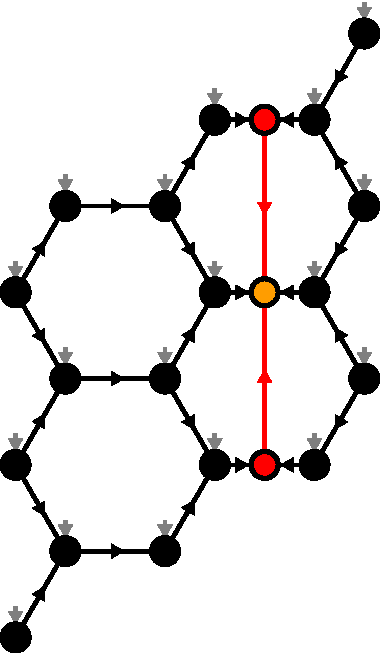
\includegraphics[scale=0.5]{figures/tikz/TFI/hexagonal_lattice/hexagonal_lattice_structure.pdf}
		}
	\end{minipage}
	\caption{In this figure we show imaginary TEBD results using disoTPS on the honeycomb lattice. We used two different values for the horizontal bond dimension, $D_\text{horizontal} = D$ and $D_\text{horizontal} = D^2$. The bond dimension along the orthogonality hypersurface was chosen as $\chi = 6\cdot D$. For the YB move we used the approximate Rényi-$0.5$ disentangler with a maximum of $N_\text{iter} = 100$ iterations per YB move. The model is the TFI model on a $4\times 4$ honeycomb lattice at a transverse field of $g = 3.5$. On the right we show the disoTPS structure of a $3\times 3$ honeycomb lattice as comparison.}
	\label{fig:tfi_gs_energy_vs_dtau_honeycomb}
\end{figure}
%
Last, to show the generalization of disoTPS to other lattice types, we implemented disoTPS on the honeycomb lattice. The network structure is shown on the right in Figure \figref{fig:tfi_gs_energy_vs_dtau_honeycomb}. For details of the implementation see \cite{}\todo{cite github}. For disoTPS on the honeycomb lattice it can be beneficial to choose a larger bond dimension $D_\text{horizontal}$ for horizontal bonds, since else the maximal bond dimension of the diagonal bonds is not reached even in the bulk, see Figure \figref{fig:honeycomb_horizontal_bond_problem}. We test this in Figure \figref{fig:tfi_gs_energy_vs_dtau_honeycomb}, where we compute the ground state energy of the TFI model on a $4\times4$ honeycomb lattice. We run the algorithm once with $D_\text{horizontal} = D$ and once with $D_\text{horizontal} = D^2$, which improves the results but also has a higher computational cost. Further testing is required to determine which bond dimension should be chosen in practice.
\begin{figure}
	\centering
	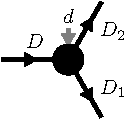
\includegraphics[scale=1]{figures/tikz/TFI/hexagonal_lattice/hexagonal_lattice_horizontal_bond_problem.pdf}
	\caption{If the maximum horizontal bond dimension of the honeycomb disoTPS is set to $D$, a physical tensor in the bulk must fulfil the isometry condition $D\cdot d \le D_1\cdot D_2$. Since most often $d < D$, the maximum bond dimension cant be reached for the outgoing legs. This can create anisotropies in the tensor network.}
	\label{fig:honeycomb_horizontal_bond_problem}
\end{figure}